\documentclass{article}
\usepackage[utf8]{inputenc}
\usepackage[siunitx, RPvoltages]{circuitikz}
\usetikzlibrary{shapes, calc}

\title{Superconducting Polychronous Computing Near Criticality: Transponder}
\author{W. Armstrong}
\date{\today}

\usepackage[english]{babel}
\usepackage{amsmath}
\usepackage{amssymb}
\usepackage{graphicx}
\usepackage[colorinlistoftodos]{todonotes}
\usepackage{pgfplots}
\pgfplotsset{compat=1.14}
\usepackage{siunitx}
\usepackage{circuitikz}

% if we ever make a custom style package for group memos
%\usepackage{qnn} 
\usepackage{palatino}
\usepackage{fancyhdr}
%\linespread{2}


\newcommand{\version}{0.2}
\fancyhf{} % sets both header and footer to nothing
\renewcommand{\headrulewidth}{0pt}
\renewcommand{\footrulewidth}{0pt}
\rhead{SPCNC Transponder v\version-\thepage}

\newcommand{\FIXME}[1]{\textit{#1}}
\newcommand{\sub}[1]{\ensuremath{_\mathrm{#1}}}
\newcommand{\kOhm}[1]{\SI{#1}{\kilo\ohm}}



\tikzset{
  nTron/.pic = {
    \draw (0,0) 
    -- ++(0,0.8) 
    -- ++(-0.4,-0.2)
    -- ++(0,1.0)
    -- ++(0.4,-0.2)
    -- ++(0,0.8);
       \draw [-{Triangle}] (-1.3,1) to (-0.4,1); 
    %(0,0) ++(-0.4,1.0) -- +(-0.8,0)
    %(0,0) ++(-0.4,1.0) -- +(-0.3,0.2)
    %(0,0) ++(-0.4,1.0) -- +(-0.3,-0.2);
    \draw[ultra thick] 
    (0,0) ++(-0.4,0.6) -- +(0,1.0);
  }
}
\tikzset{
  heaterTron/.pic = {
    \draw (0,0)     % channel lead 1 at (#1,#2)
    % channel lead 2 at (#1,#2+2.2)
    -- ++(0,0.8) 
    -- ++(-0.4,-0.2)
    -- ++(0,1.0)
    -- ++(0.4,-0.2)
    -- ++(0,0.8)
    %bottom heater lead node (#1-1.4,#2+0.7)
    (0,0) ++(-1.4,0.7 ) -- ++(0.8,0)
    %top heater lead (#1-1.4,#2+1.5)
    ++(0,0.8)
    -- ++(-0.8,0);
    %channel
    \draw[ultra thick] (0,0) ++(-0.4,0.6) -- +(0,1.0);
    %heater
    \draw[ultra thick] (0,0) ++(-0.6,0.7) -- +(0,0.8);
  }
}
\tikzset{
  tronChannel/.pic = {
    \draw (0,0)     % channel lead 1 at (#1,#2)
    % channel lead 2 at (#1,#2+2.2)
    -- ++(0,0.8) 
    -- ++(-0.4,-0.2)
    -- ++(0,1.0)
    -- ++(0.4,-0.2)
    -- ++(0,0.8);
    %channel
    \draw[ultra thick] (0,0) ++(-0.4,0.6) -- +(0,1.0);
  }
}
\tikzset{
  yTron/.pic = {
    \draw (0,0) 
    -- ++(0,0.8) 
    -- ++(-0.4,-0.2)
    -- ++(0,1.0)
    -- ++(0.4,-0.2)
    -- ++(0,0.8)
    (0,0) ++(-0.4,1.2) ++(-0.4,0.4) -- +(-0.4,0);
    \draw[ultra thick] (0,0) ++(-0.4,1.2) -- +(-0.4,0.4);
    \draw[ultra thick] (0,0) ++(-0.4,0.6) -- +(0,1.0);
  }
}

\newcommand{\ie}{i.e.}
\newcommand{\eg}{e.g.}

\newcommand{\Lo}{\ensuremath{L\sub{\circ}}}
\newcommand{\isw}{\ensuremath{i\sub{sw}}}
\newcommand{\Tw}{\ensuremath{T\sub{w}}}

\begin{document}

\maketitle

\section{Introduction}





\begin{figure}[htb!]
  \centering
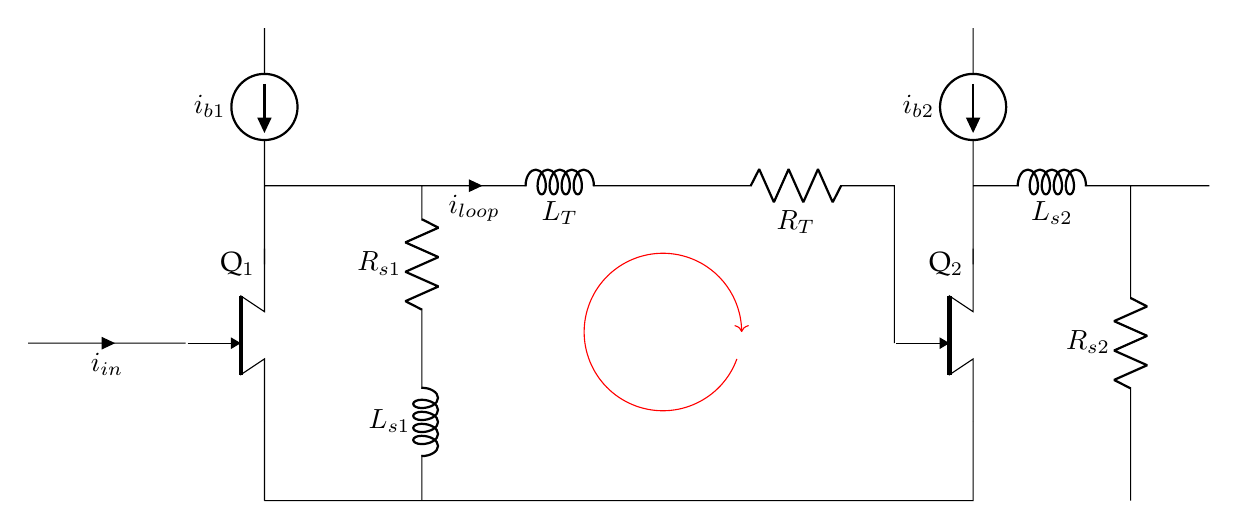
\begin{tikzpicture}[scale=2]
  \draw[color=black]
    (0,3) to [american current source,l_=$i_{b1}$] (0,2) 
    (0,0) to (0,0.5) 
    pic [xscale=0.75, scale=0.5,transform shape] {nTron} (0,1.5) node [left] {Q$_1$}
    to (0,2)
    to (1,2)
    to [R,l_=$R_{s1}$] (1,1)
    to [L,l_=$L_{s1}$] (1,0)
    (-1.5,1) to [short,i>_=$i_{in}$] (-0.5,1)
    (1,2)  
    to [L,l_=$L_{T}$,i>_=$i_{loop}$] (2.75,2)
    to [R,l_=$R_{T}$] (4,2) 
    to (4,1) 
    (4.5,0.5)
    pic [xscale=0.75, scale=0.5,transform shape]  {nTron} (4.5,1.5) node [left] {Q$_2$}
    (4.5,3) to [american current source,l_=$i_{b2}$] (4.5,2) 
    (4.5,0.5)
    to (4.5,0)
    to (0,0) 
    (4.5,1.5)
    to (4.5,2) 
    to (4.5,2) 
    to [L,l_=$L_{s2}$] (5.5,2)
    to [R,l_=$R_{s2}$] (5.5,0) 
    (5.5,2) to (6,2) [open] {} ; 

  \draw[->,red] (3,0.9) arc [radius=0.5cm,start angle=340,end angle=0];
\end{tikzpicture}
\caption{Transponder circuit.\label{fig:transponder}}
\end{figure}

\section{Transponder Model}

A simplified circuit for modeling the internal loop current is shown in Figure~\ref{fig:circuit2}.
There are some issues for modeling: 
\begin{itemize}
  \item Input and output isolation 
  \item Details of ntron switching model
\end{itemize}
 
\begin{figure}[htb!]
  \centering
  \ctikzset{bipoles/length=.9cm}
  \begin{circuitikz}[scale=2]
  %\ctikzset{resistors/scale=0.8, capacitors/scale=0.7, diodes/scale=0.6, transistors/scale=1.3}
  \draw[color=black]
    (0,3) to [american current source,l_=$i_{b1}$] (0,2) 
    %(0,0) to (0,0.5) 
    %pic [xscale=0.75, scale=0.5,transform shape] {nTron} (0,1.5) node [left] {nT$_1$}
    to [R,l_=$R_{nw}(i_g) $,i>_=$i_{nw}$] (0,1)
    to [L,l_=$L_{nw}$] (0,0)
    (0,2)
    to (1,2)
    to [R,l_=$R_{s1}$,i>_=$i_{s1}$] (1,1)
    to [L,l_=$L_{s1}$] (1,0)
    (1,2)
    to (2,2)
    to [R,l_=$R_{T}$,i>_=$i_{loop}$] (2,1)
    to [L,l_=$L_{T}$] (2,0) 
    to (0,0);
\end{circuitikz}
\caption{Simplified circuit.\label{fig:circuit2}}
\end{figure}

From current conservation we have $i_{b1} = i_{nw} + i_{s1} + i_{loop}$  and going around the loops:
\begin{equation} \label{tloop1}
  \begin{split}
    L_{nw} \frac{d i_{nw}}{dt} + i_{nw} R_{nw}(t) &= i_{s1} +R_{s1} + L_{s1} \frac{d i_{s1}}{dt} \\
                                                  &= (i_{1} - i_{nw} - i_{loop} )R_{s1} - L_{s1} \Big(\frac{d i_{nw}}{dt} + \frac{d i_{loop}}{dt}\Big)
  \end{split}
\end{equation}

\begin{equation} \label{tloop2}
    L_{nw} \frac{d i_{nw}}{dt} + i_{nw} R_{nw}(t) = i_{loop} +R_{T} + L_{T} \frac{d i_{loop}}{dt} 
\end{equation}

These reduce to coupled differential equations for the unknown currents through the input ntron channel $i_{nw}$ and the loop current $i_{loop}$. 
\begin{multline}
  \frac{di_{nw}}{dt} =  \frac{-i_{nw} L_{s1} R_{nw} - i_{1} L_T R_{s1} + i_{loop} L_T R_{s1} + i_{nw} L_{T} (R_{nw} + R_{s1}) + i_{loop} L_{s1} R_T}{L_{nw} (L_{s1} - L_T) - L_{s1} L_T}
\end{multline}
\begin{multline}
  \frac{di_{loop}}{dt} =  \frac{-i_{nw} L_{s1} R_{nw} - i_{1} L_{nw} R_{s1} + i_{loop} L_{nw} R_{s1} + i_{nw} L_{nw} R_{s1} + i_{loop} L_{nw} R_T + i_{loop} L_{s1} R_T}{L_{nw} (L_{s1} - L_T) - L_{s1} L_T}
\end{multline}
Connected to the output nTron's gate, the loop current causes the output of the transponder to fire one the threshold current is reached.
This is not included in the simple model above which only injects current into the leaky current loop.
For a first crude and simple model of the input nTron  Q$_1$ firing, the nTron is modeled as a variable resistance which is a linear spike.

\subsection{Modeling $R_{nw}$}
The resistance is turned on for a few nanoseconds :
\begin{equation}
R(t; t_0) = 
    \begin{cases}
        R_0 (t-t_0+t_r)/t_r & \text{if } -t_r < (t-t_0) <0 \\
        R_0 & \text{if } 0 <  (t-t_0) < t_w \\
        R_0 (t_f-(t-t_0 -t_w))/t_f & \text{if } t_w < (t-t_0) < t_w + t_f  \\
        0 
    \end{cases}
\end{equation}


\begin{figure}[htb]
  \centering
  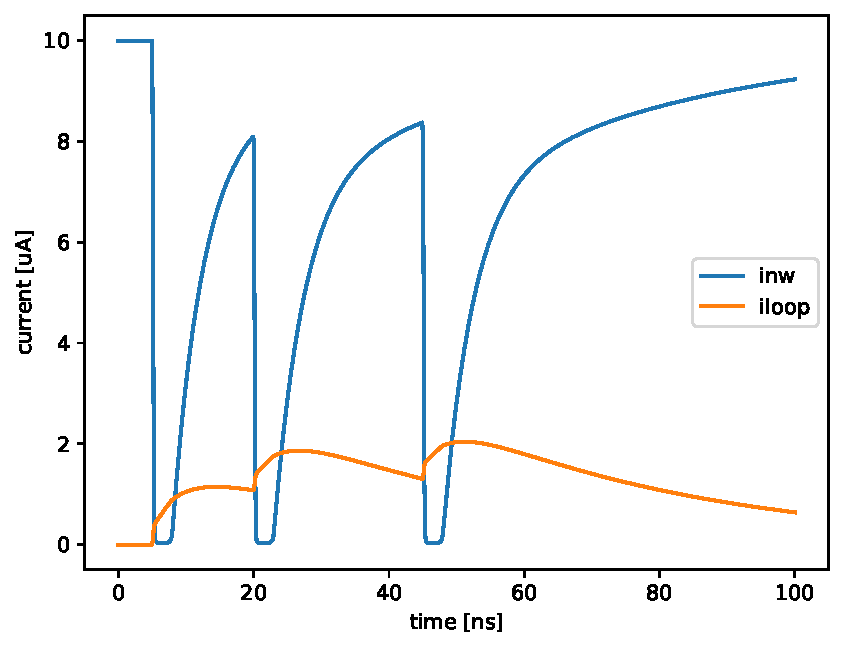
\includegraphics[width=0.7\textwidth]{figs/current_loop.pdf}
  \caption{\label{fig:loopcurrentmodel} Stored loop current for 3 input pulses in the simple model.}
\end{figure}

\section{Transponder Output}

The output ntron is one of two controls for each transponder. The output circuit shown in Figure~\ref{fig:circuit3}
shows the model of the ntron as a variable resistance and the inputs to downstream transponders as terminated delay lines.
Rather than solving the system of equations for each output configuration, 
we assume that the output current is divided among the $n$ output connections, each with the same characteristic impedance.
Thus, the output current is split N-ways and the stiff voltage divider formed by the relatively low shut impedance 
($R_{s2}$ and $L_{s2}$) shapes the output pulse.

For the sake of simplicity, the shape of the output pulse is a model that is scaled depending on the number of output connections.



\begin{figure}[htb!]
  \centering
  \ctikzset{bipoles/length=.9cm}
  \begin{circuitikz}[scale=2]
  %\ctikzset{resistors/scale=0.8, capacitors/scale=0.7, diodes/scale=0.6, transistors/scale=1.3}
  \draw[color=black]
    (0,3) to [american current source,l_=$i_{b2}$] (0,2) 
    %(0,0) to (0,0.5) 
    %pic [xscale=0.75, scale=0.5,transform shape] {nTron} (0,1.5) node [left] {nT$_1$}
    to [R,l_=$R_{nw}(i_g) $,i>_=$i_{nw}$] (0,1)
    to [L,l_=$L_{nw}$] (0,0)
    (0,2)
    to [L,l^=$L_{out}$] (1,2)
    to [L,l_=$L_{s2}$,i>_=$i_{s2}$] (1,1)
    to [R,l_=$R_{s2}$] (1,0)
    to (0,0)
    (1,2)
    to (2,2)
    (2,3)
    to (2,1);
  \draw[color=black] (2,1)
    to [TL,name=tl1,l^=$Z_0$]              (3,1) to [R,l_=$R_{1}$,i>_=$i_{1}$] (4,1) to [L,l_=$L_{1}$] (5,1) 
    (2,2)
    to [TL,bipoles/tline/width=1,l^=$Z_0$] (3,2) to [R,l_=$R_{2}$,i>_=$i_{2}$] (4,2) to [L,l_=$L_{2}$] (5,2) 
    (2,3)
    to [TL,bipoles/tline/width=2,l^=$Z_0$] (3,3) to [R,l_=$R_{3}$,i>_=$i_{3}$] (4,3) to [L,l_=$L_{3}$] (5,3) 
    ;
  \draw (5,1) -- ++(0,-0.1) node [tlground]{};
  \draw (5,2) -- ++(0,-0.1) node [tlground]{};
  \draw (5,3) -- ++(0,-0.1) node [tlground]{};
\end{circuitikz}
\caption{Output circuit with variable delay transmission lines \label{fig:circuit3}}
\end{figure}

\subsection{Non-ideal Behavior}

The circuit shown in Figure~\ref{fig:circuit4} shows the terminating end of one of the inputs ($i_2$) as it looks 
when the input ntron is firing. If a pulse arrives at this time then reflections will likely occur. 
Furthermore, the corresponding channel current that is being shunted (not shown) has a path to ground through that output branch 
rather than  $R_{gs}$ of the firing ntron. The low shunt impedance, $(n-1)$ output connections, and $L_{out}$ 
should help mitigate this behavior.

\textcolor{red}{Todo: look into these issues with spice simulations.}

\begin{figure}[htb!]
  \centering
  \ctikzset{bipoles/length=.9cm}
\begin{circuitikz}[ scale = 2 ]
  \draw[color=black]
    (0,3) to [american current source,l_=$i_{b2}$] (0,2) 
    %(0,0) to (0,0.5) 
    %pic [xscale=0.75, scale=0.5,transform shape] {nTron} (0,1.5) node [left] {nT$_1$}
    to [R,l_=$R_{nw}(i_g) $,i>_=$i_{nw}$] (0,1)
    to [L,l_=$L_{nw}$] (0,0)
    (0,2)
    to [L,l^=$L_{out}$] (1,2)
    to [L,l_=$L_{s2}$,i>_=$i_{s2}$] (1,1)
    to [R,l_=$R_{s2}$] (1,0)
    to (0,0)
    (1,2)
    to (2,2)
    (2,3)
    to (2,1);
  \draw[color=black] (2,1)
    to [TL,name=tl1,l^=$Z_0$] (3,1) to [R,l_=$R_{1}$,i>_=$i_{1}$] (4,1) to [L,l_=$L_{2}$] (5,1) 
    (2,2)
    to [TL,bipoles/tline/width=1,l^=$Z_0$] (3,2) to [R,l_=$R_{2}$,i>_=$i_{2}$] (4,2) to [L,l_=$L_{2}$] (5,2) 
    (2,3)
    to [TL,bipoles/tline/width=2] (3,3) to [R,l_=$R_{4}$,i>_=$i_{3}$] (4,3) to [L,l_=$L_{3}$] (5,3) 
    ;
  \draw (5,1) -- ++(0,-0.1) node [tlground]{};
  \draw (5,2) to [R,l^=$R_{gs}$] (5,1.5)  node [tlground]{};
  \draw (5,3) -- ++(0,-0.1) node [tlground]{};
\end{circuitikz}
\caption{Example showing temporary high impedance and possibly a source of leaking channel current into output circuit when a connected transponder's input ntron fires.\label{fig:circuit4}}
\end{figure}

\section{Transponder Input}

\textcolor{red}{Need a simple relation between $i_{b1}$ and $I_{SW}$}

\begin{figure}[htb]
  \centering
  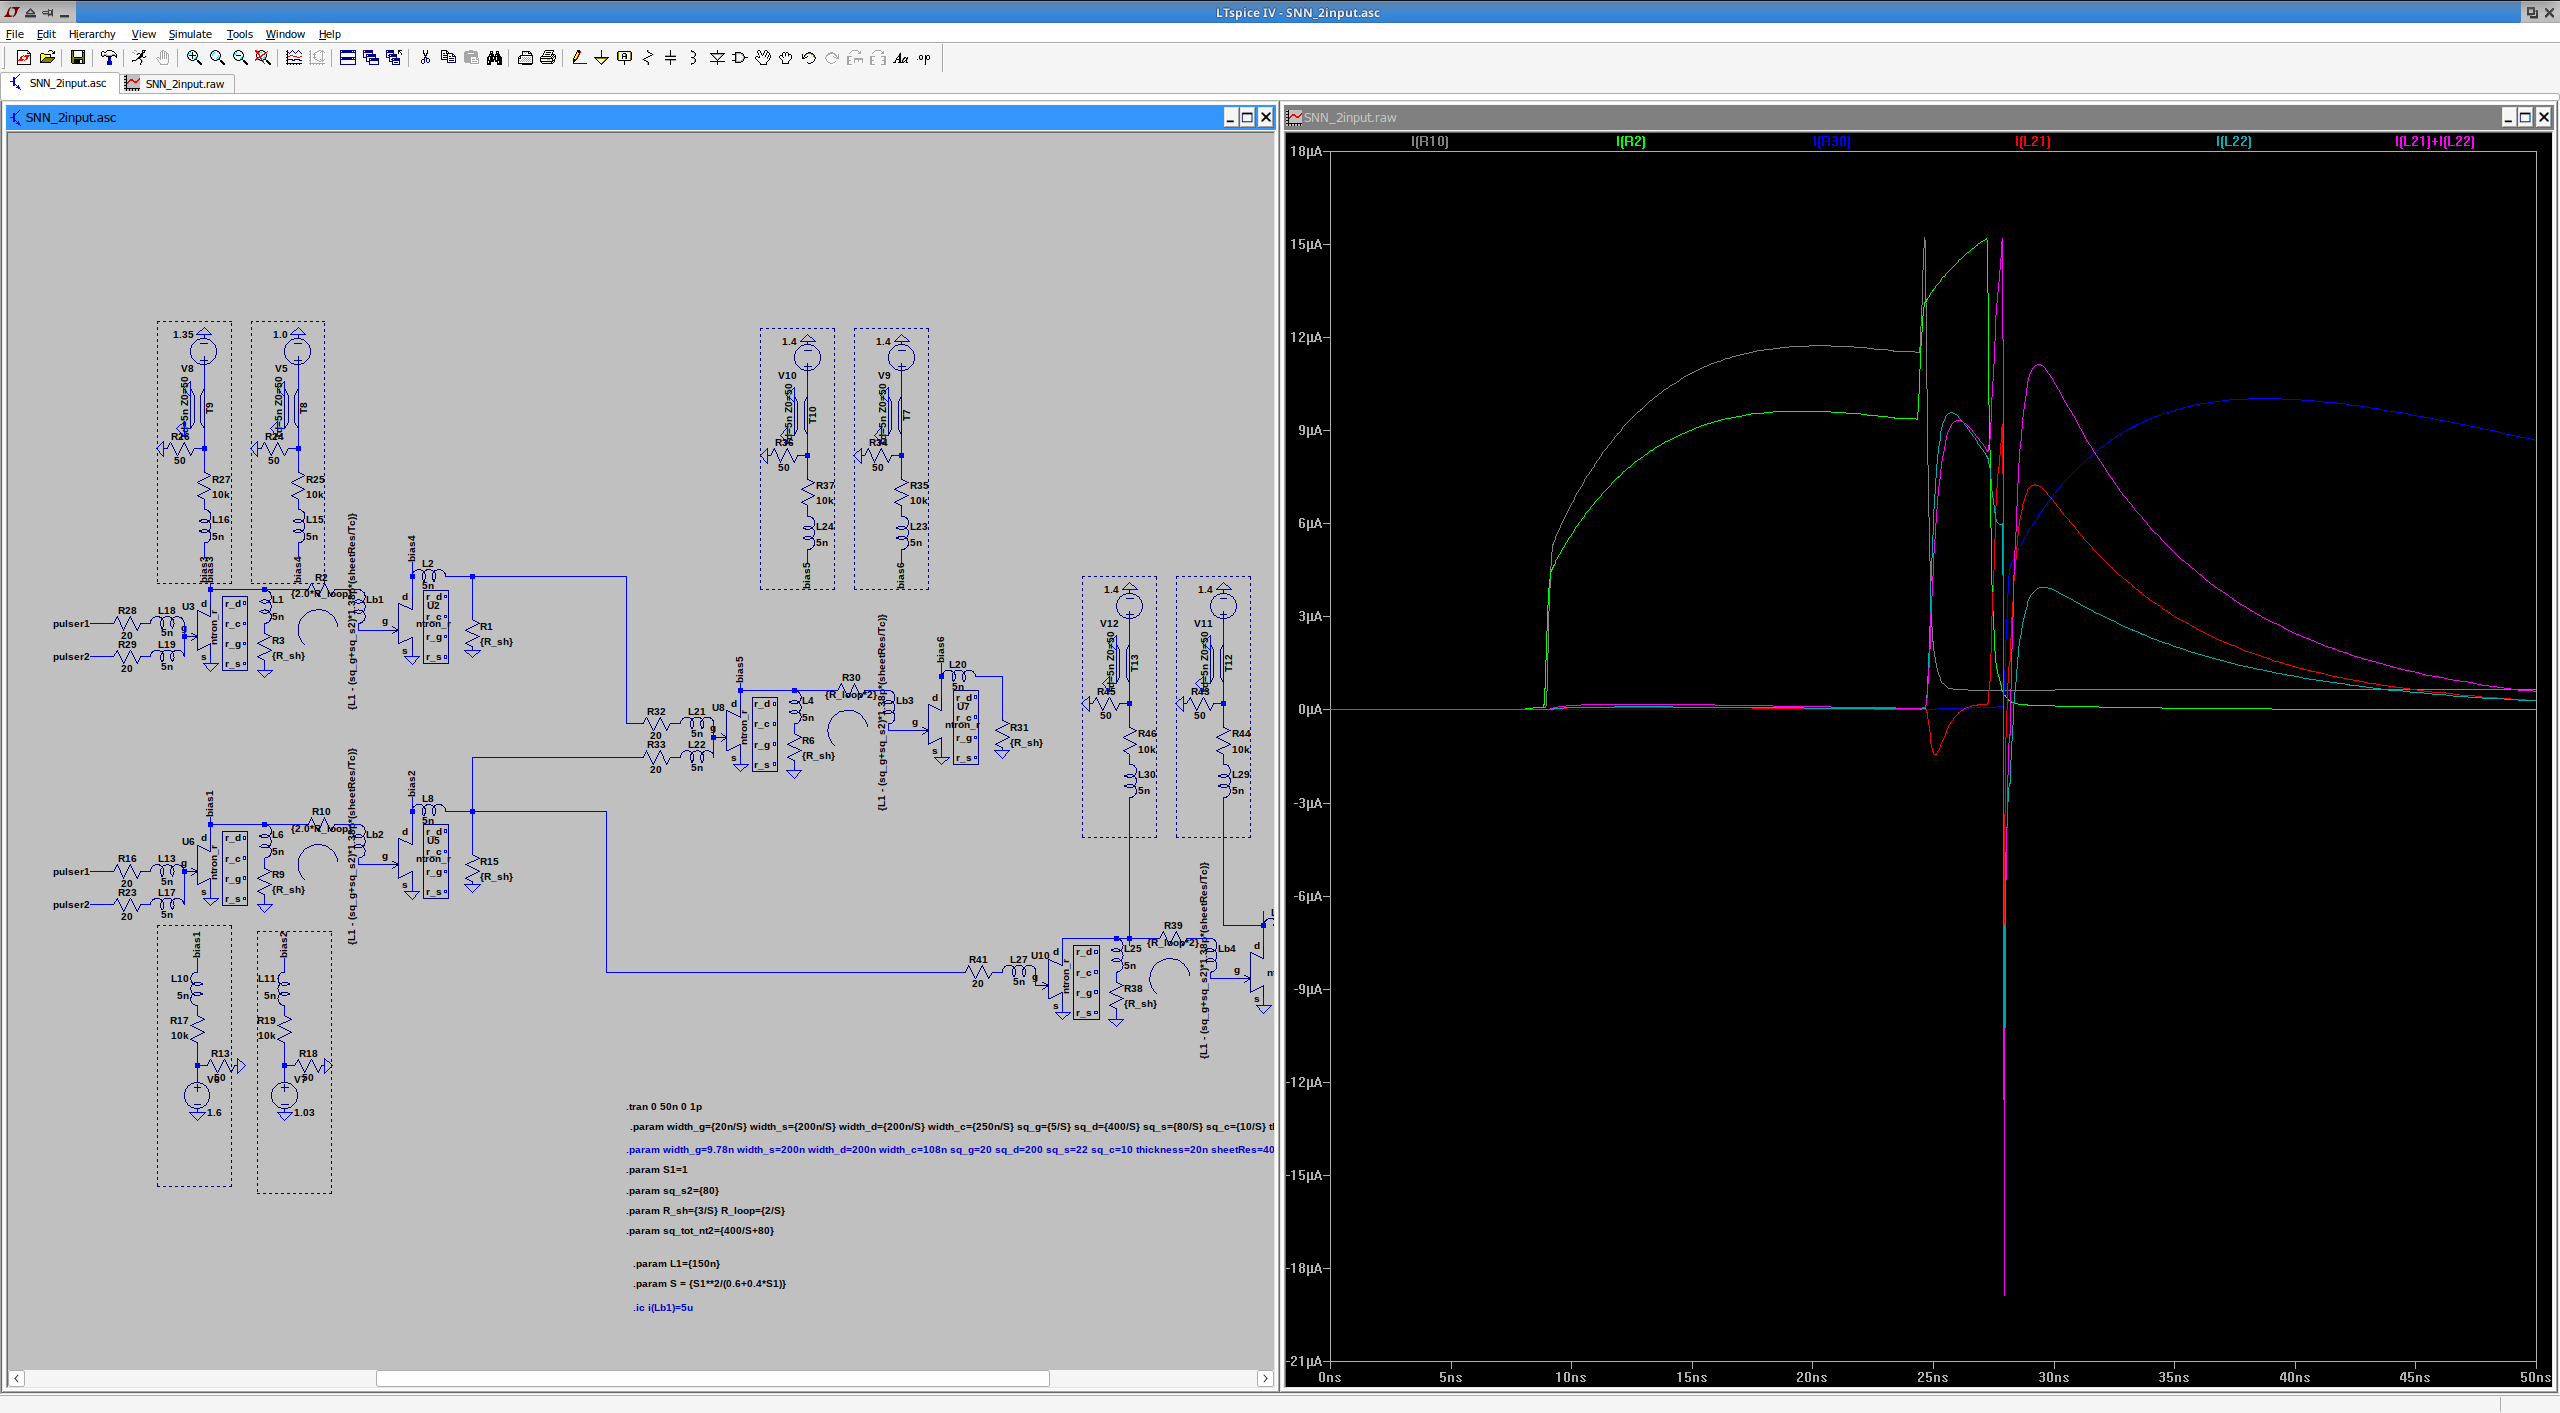
\includegraphics[width=1.0\textwidth,clip,trim=100mm 50mm 0mm 50mm]{figs/input_sum_above_n2_fanout.png}\\
  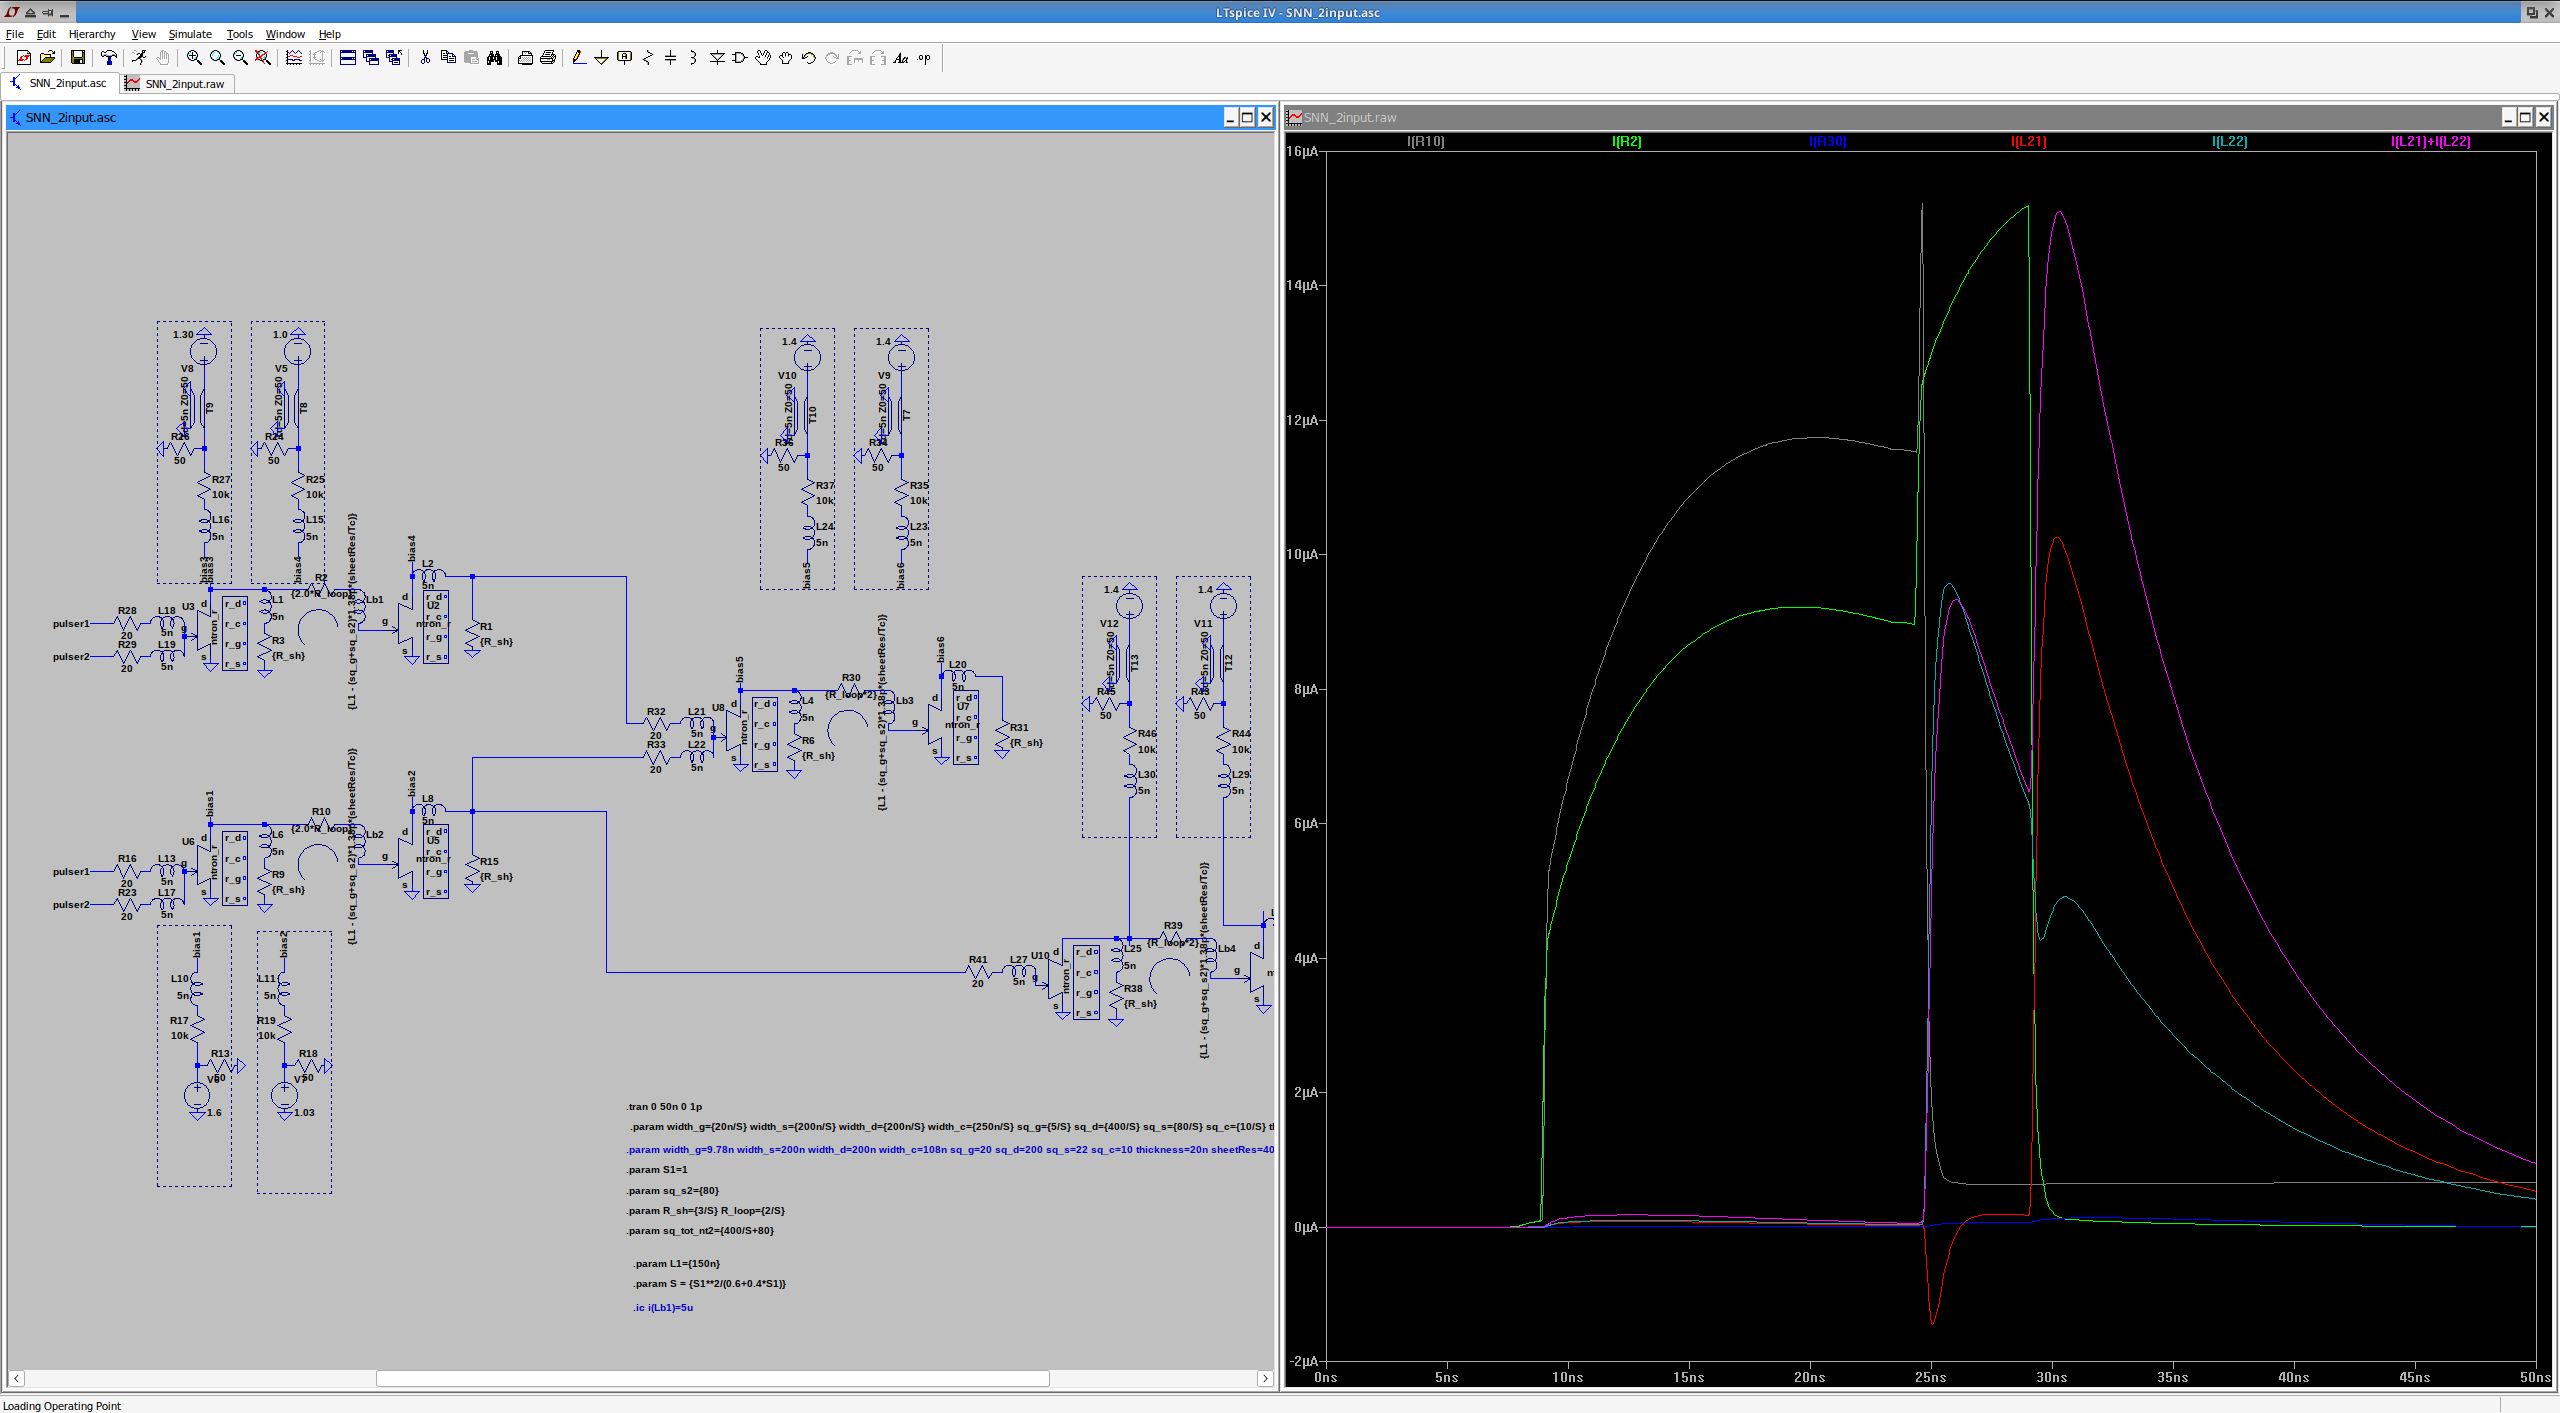
\includegraphics[width=1.0\textwidth,clip,trim=100mm 50mm 0mm 50mm]{figs/input_sum_below_n2_fanout.png}\\
  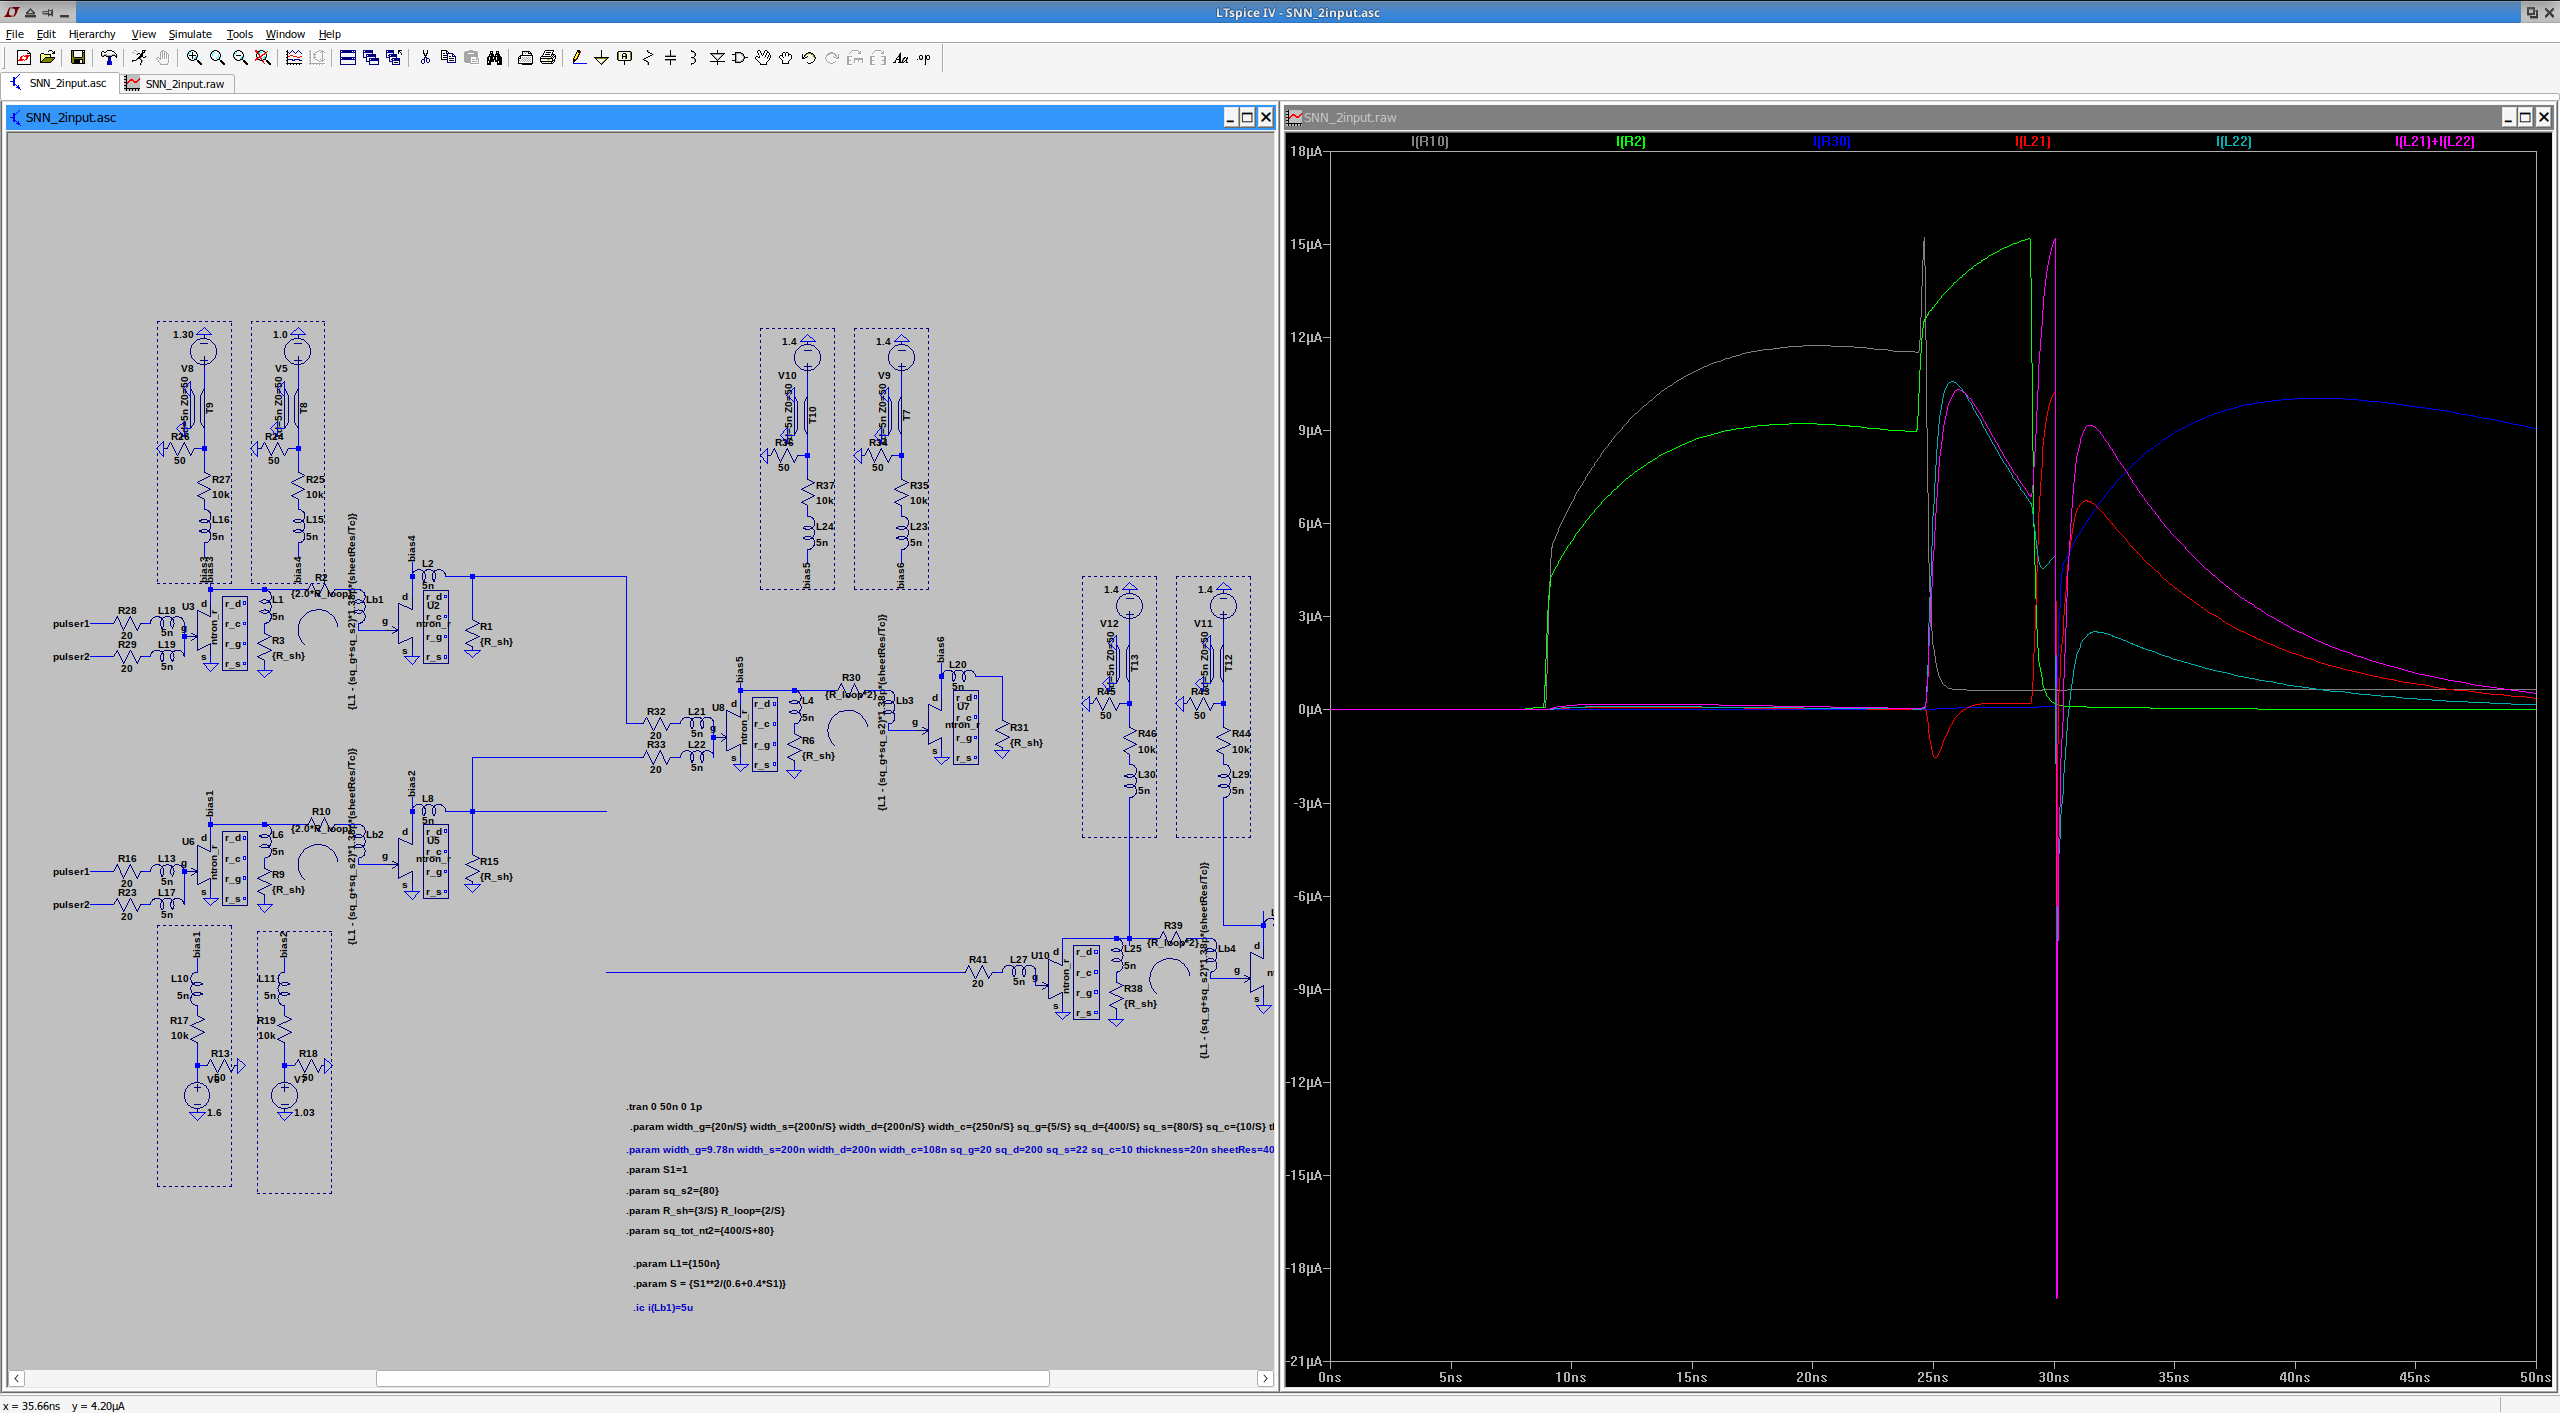
\includegraphics[width=1.0\textwidth,clip,trim=100mm 50mm 0mm 50mm]{figs/input_sum_above_no_n2_fanout.png}
  \caption{\label{fig:inputsum}(Top) Input from two pulses add together causing the input current to go above threshold. 
    (Middle) Same as above but with delayed second pulse arrival, input current stays below threshold, and
  (Bottom) removing output load on upstream input increases current enough that downstream input  current goes above threshold again.  }
\end{figure}


\section{Network Connectivity} 


\subsection{Transmission Line}

Using a coplanar wave guide calculator:
Silicon relative dielectric constant $\epsilon_r = 11.9 $,
Dielectric loss $\tan \delta = 0.015$,

Width of \qty{2}{\um}  and spacing of 0.2 um gives $Z_0 = $ \qty{29}{\ohm}. 

Width of \qty{0.2}{\um} and spacing of \qty{1}{\mu} gives $Z_0=$ \qty{93}{\ohm}.

Width of \qty{0.4}{\um} and spacing of \qty{1}{\mu} gives $Z_0=$ \qty{78}{\ohm}.

Width of \qty{1}{\um} and spacing of \qty{1}{\mu} gives $Z_0=$ \qty{60}{\ohm}.

\begin{figure}[htb]
  \centering
  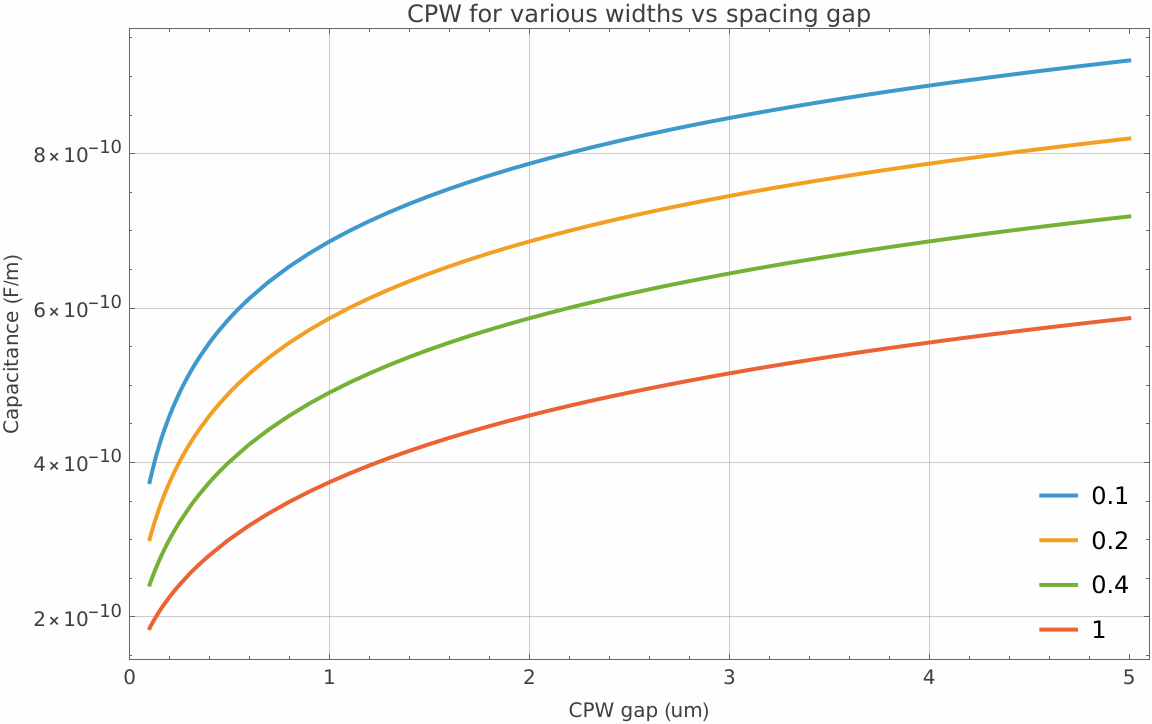
\includegraphics[width=1.0\textwidth,clip,trim=0mm 0mm 0mm 0mm]{CPW_capacitance.png}
  \caption{\label{fig:cpwcap}Coplanar waveguide Capacitance per unit length for various wire widths. }
\end{figure}
\begin{figure}[htb]
  \centering
  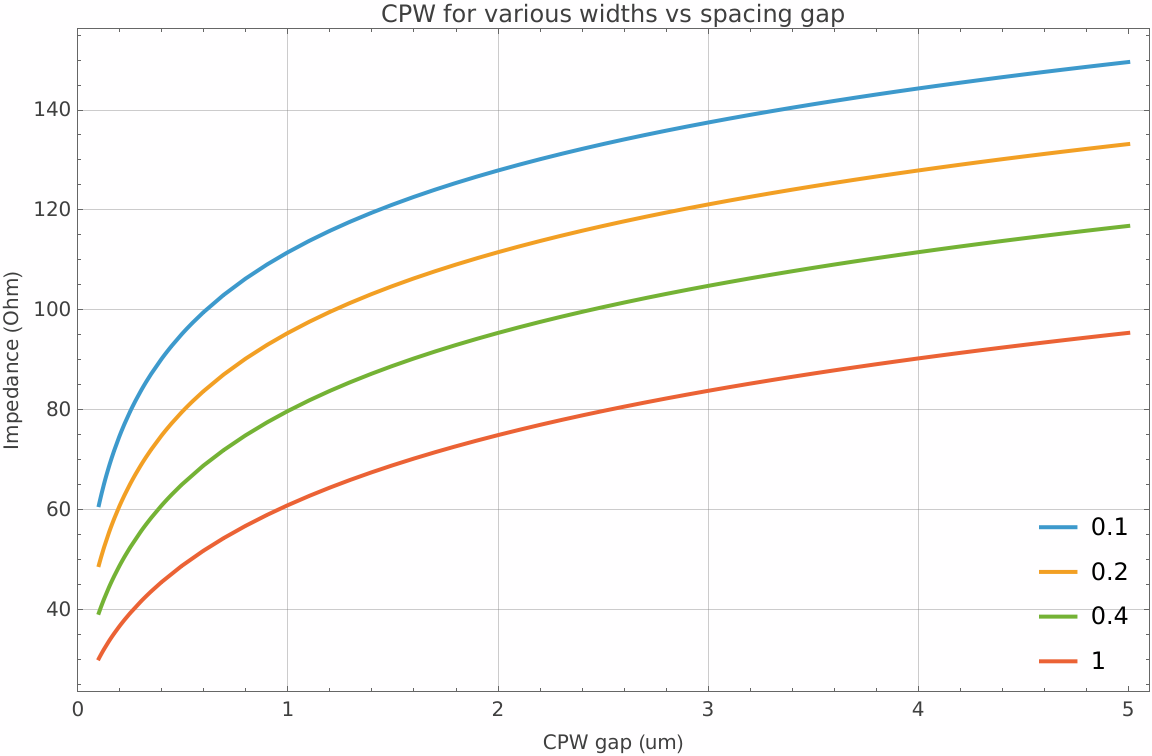
\includegraphics[width=1.0\textwidth,clip,trim=0mm 0mm 0mm 0mm]{CPW_Z0.png}
  \caption{\label{fig:cpwcap}Coplanar waveguide impedance for various wire widths. }
\end{figure}


\appendix

\section{Criticality} 
\begin{figure}[htb]
  \centering
  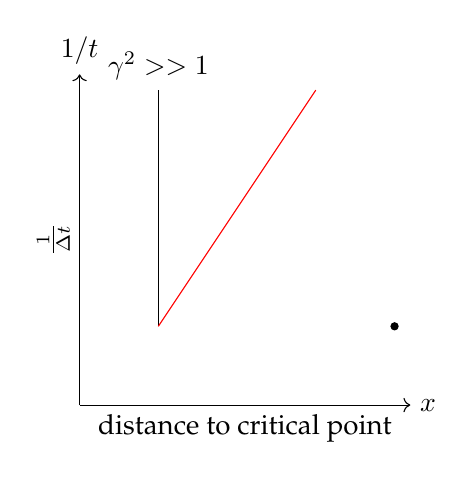
\begin{tikzpicture}[domain=1:4]
    %\draw[very thin,color=gray] (-0.1,-1.1) grid (3.9,3.9);

    \draw[->] (0,0) -- (4.2,0) node[midway,below]{distance to critical point } node[right] {$x$};
    \draw[->] (0,0) -- (0,4.2) node[midway,above,rotate=90]{ $ \frac{1}{\Delta t}$}  node[above] {$1/t$};

    \fill[black] (4,1) circle(1.5pt) {} ;
    \draw[color=black]  plot[domain=0:1] (1     ,3*\x+1)  node[above] {$\gamma^2 >> 1$};
    \draw[color=red]    plot[domain=0:1] (1+2*\x,3*\x+1)  node[right] { };
    % \x r means to convert '\x' from degrees to _r_adians:
    %\draw[color=blue]   plot (\x,{1/(1-0.05*\x*\x)})    node[right] {$f(x) = \sin x$};
    %\draw[color=blue] plot (\x,{0.05*exp(\x)}) node[right] {$f(x) = \frac{1}{20} \mathrm e^x$};
  \end{tikzpicture}
  \caption{\label{fig:crit} Distance to critical point on x axis.}
\end{figure}


\end{document}


